\documentclass[conference]{IEEEtran}
\IEEEoverridecommandlockouts
% The preceding line is only needed to identify funding in the first footnote. If that is unneeded, please comment it out.
\usepackage{cite}
\usepackage{amsmath,amssymb,amsfonts}
\usepackage{graphicx}
\usepackage{textcomp}
\usepackage{xcolor}
\usepackage[hyphens]{url}
\usepackage{hyperref}
\usepackage{listings}
\def\BibTeX{{\rm B\kern-.05em{\sc i\kern-.025em b}\kern-.08em
    T\kern-.1667em\lower.7ex\hbox{E}\kern-.125emX}}

\newcommand{\rom}[1]{\uppercase\expandafter{\romannumeral #1\relax}}

\begin{document}

\onecolumn


\title{HackTheBox: WhatIsIt?}

\author{\IEEEauthorblockN{Lennart Buhl}
\IEEEauthorblockA{\textit{Department of Computer Science} \\
\textit{University of St. Thomas}\\
\textit{September, 2023}}}

\maketitle



\begin{abstract}

\end{abstract}



\begin{IEEEkeywords}
programming, cybersecurity, security, pentesting
\end{IEEEkeywords}


\section{Introduction}
Redeemer is located at IPv4 10.129.23.6. Which we can access through the HackTheBox OpenVPN gateway.
We achieve this by simply running this command in a shell:
\begin{scriptsize}
\begin{verbatim}
sudo openvpn starting_point_{user}.ovpn
\end{verbatim}
\end{scriptsize}

\\
\textit{We will now switch to root shell.}
\\

Once we are on the VPN, we scan the machine via nmap:
\begin{scriptsize}
\begin{verbatim}
root@ghost:~# nmap -p- -sC -sV 10.129.23.6
Starting Nmap 7.94 ( https://nmap.org ) at 2023-09-09 16:42 CDT
Nmap scan report for 10.129.23.6
Host is up (0.065s latency).
Not shown: 65533 closed tcp ports (reset)
PORT   STATE SERVICE VERSION
21/tcp open  ftp     vsftpd 3.0.3
| ftp-syst:
|   STAT:
| FTP server status:
|      Connected to ::ffff:10.10.16.108
|      Logged in as ftp
|      TYPE: ASCII
|      No session bandwidth limit
|      Session timeout in seconds is 300
|      Control connection is plain text
|      Data connections will be plain text
|      At session startup, client count was 3
|      vsFTPd 3.0.3 - secure, fast, stable
|_End of status
| ftp-anon: Anonymous FTP login allowed (FTP code 230)
| -rw-r--r--    1 ftp      ftp            33 Jun 08  2021 allowed.userlist
|_-rw-r--r--    1 ftp      ftp            62 Apr 20  2021 allowed.userlist.passwd
80/tcp open  http    Apache httpd 2.4.41 ((Ubuntu))
|_http-title: Smash - Bootstrap Business Template
|_http-server-header: Apache/2.4.41 (Ubuntu)
Service Info: OS: Unix

Service detection performed. Please report any incorrect results at https://nmap.org/submit/ .
Nmap done: 1 IP address (1 host up) scanned in 22.37 seconds
\end{verbatim}
\end{scriptsize}

We can see we have a webpage and a file server. We should first check out the webpage to see what we have there.



\begin{figure}[htb]

\includegraphics[scale=0.075]{business_digital.png}
\centering
\end{figure}

As we can see, just a simple webpage. Let's check out the file server:


\begin{scriptsize}
\begin{verbatim}
root@ghost:~# ftp -a 10.129.23.6
Connected to 10.129.23.6.
220 (vsFTPd 3.0.3)
230 Login successful.
Remote system type is UNIX.
Using binary mode to transfer files.
ftp> ls
229 Entering Extended Passive Mode (|||42324|)
150 Here comes the directory listing.
-rw-r--r--    1 ftp      ftp            33 Jun 08  2021 allowed.userlist
-rw-r--r--    1 ftp      ftp            62 Apr 20  2021 allowed.userlist.passwd
226 Directory send OK.
ftp> get allowed.userlist
local: allowed.userlist remote: allowed.userlist
229 Entering Extended Passive Mode (|||44599|)
150 Opening BINARY mode data connection for allowed.userlist (33 bytes).
100% |************************************************************************|    33        0.39 KiB/s    00:00 ETA
226 Transfer complete.
33 bytes received in 00:00 (0.20 KiB/s)
ftp> get allowed.userlist.passwd
local: allowed.userlist.passwd remote: allowed.userlist.passwd
229 Entering Extended Passive Mode (|||42021|)
150 Opening BINARY mode data connection for allowed.userlist.passwd (62 bytes).
100% |************************************************************************|    62        0.81 KiB/s    00:00 ETA
226 Transfer complete.
62 bytes received in 00:00 (0.34 KiB/s)
ftp> exit
221 Goodbye.
\end{verbatim}
\end{scriptsize}

We accessed the ftp server via the "-a" flag, which allows us to access the data anonymously. We then used the "ls" commnand to list everything on the server.
    And we are presented with two files:


\begin{scriptsize}
\begin{verbatim}
ftp> ls
229 Entering Extended Passive Mode (|||42324|)
150 Here comes the directory listing.
-rw-r--r--    1 ftp      ftp            33 Jun 08  2021 allowed.userlist
-rw-r--r--    1 ftp      ftp            62 Apr 20  2021 allowed.userlist.passwd
ftp>
\end{verbatim}
\end{scriptsize}


We then use the "get" command to download the files:

\begin{scriptsize}
\begin{verbatim}
ftp> get allowed.userlist
local: allowed.userlist remote: allowed.userlist
229 Entering Extended Passive Mode (|||44599|)
150 Opening BINARY mode data connection for allowed.userlist (33 bytes).
100% |************************************************************************|    33        0.39 KiB/s    00:00 ETA
226 Transfer complete.
33 bytes received in 00:00 (0.20 KiB/s)
ftp> get allowed.userlist.passwd
local: allowed.userlist.passwd remote: allowed.userlist.passwd
229 Entering Extended Passive Mode (|||42021|)
150 Opening BINARY mode data connection for allowed.userlist.passwd (62 bytes).
100% |************************************************************************|    62        0.81 KiB/s    00:00 ETA
226 Transfer complete.
62 bytes received in 00:00 (0.34 KiB/s)
ftp>
\end{verbatim}
\end{scriptsize}

Once we have done that, we exit the ftp server and we can use the "cat" command to display the contents of both files.

\begin{scriptsize}
\begin{verbatim}
root@ghost:~# cat allowed.userlist
aron
pwnmeow
egotisticalsw
admin

root@ghost:~# cat allowed.userlist.passwd
root
Supersecretpassword1
@BaASD&9032123sADS
rKXM59ESxesUFHAd
\end{verbatim}
\end{scriptsize}


Now, we apparently have the login info something. We will now use GoBuster\cite{gobuster}\cite{seclists}, to check if there are any directories that have a login on the webpage.


\begin{scriptsize}
\begin{verbatim}
root@ghost:~# gobuster dir --url http://10.129.23.6/ --wordlist /home/francis/SecLists/Discovery/Web-Content/directory-list-2.3-small.txt
===============================================================
Gobuster v3.6
by OJ Reeves (@TheColonial) & Christian Mehlmauer (@firefart)
===============================================================
[+] Url:                     http://10.129.23.6/
[+] Method:                  GET
[+] Threads:                 10
[+] Wordlist:                /home/francis/SecLists/Discovery/Web-Content/directory-list-2.3-small.txt
[+] Negative Status codes:   404
[+] User Agent:              gobuster/3.6
[+] Timeout:                 10s
===============================================================
Starting gobuster in directory enumeration mode
===============================================================
/assets               (Status: 301) [Size: 311] [--> http://10.129.23.6/assets/]
/css                  (Status: 301) [Size: 308] [--> http://10.129.23.6/css/]
/js                   (Status: 301) [Size: 307] [--> http://10.129.23.6/js/]
/fonts                (Status: 301) [Size: 310] [--> http://10.129.23.6/fonts/]
/dashboard            (Status: 301) [Size: 314] [--> http://10.129.23.6/dashboard/]
Progress: 45685 / 87665 (52.11%)^C
[!] Keyboard interrupt detected, terminating.
Progress: 45685 / 87665 (52.11%)
===============================================================
Finished
===============================================================
\end{verbatim}
\end{scriptsize}

As we are iterating through the wordlist and testing if the directories exist, we can test the already found directories. We get prompted with a login page on the "dashboard" directory.
We then prematurely stopped gobuster, which is perhaps not recommended.

\begin{figure}[htb]
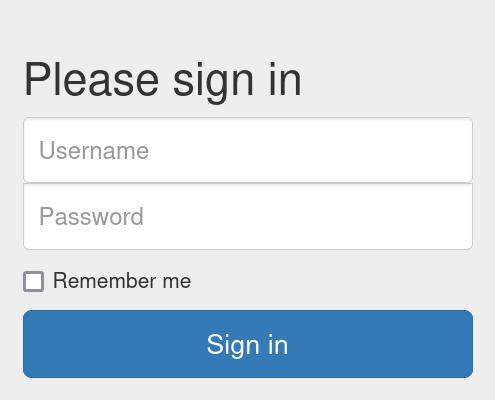
\includegraphics[scale=0.3]{login.png}
\centering
\end{figure}

We then use the user and password lists to manually try each username and password mapping. The correct combination is number 4.


\begin{scriptsize}
\begin{verbatim}
1) aron          - root
2) pwnmeow       - Supersecretpassword1
3) egotisticalsw - @BaASD&9032123sADS
4) admin         - rKXM59ESxesUFHAd
\end{verbatim}
\end{scriptsize}


Once we have entered the correct username/password mapping, we get to a new page:


\begin{figure}[htb]
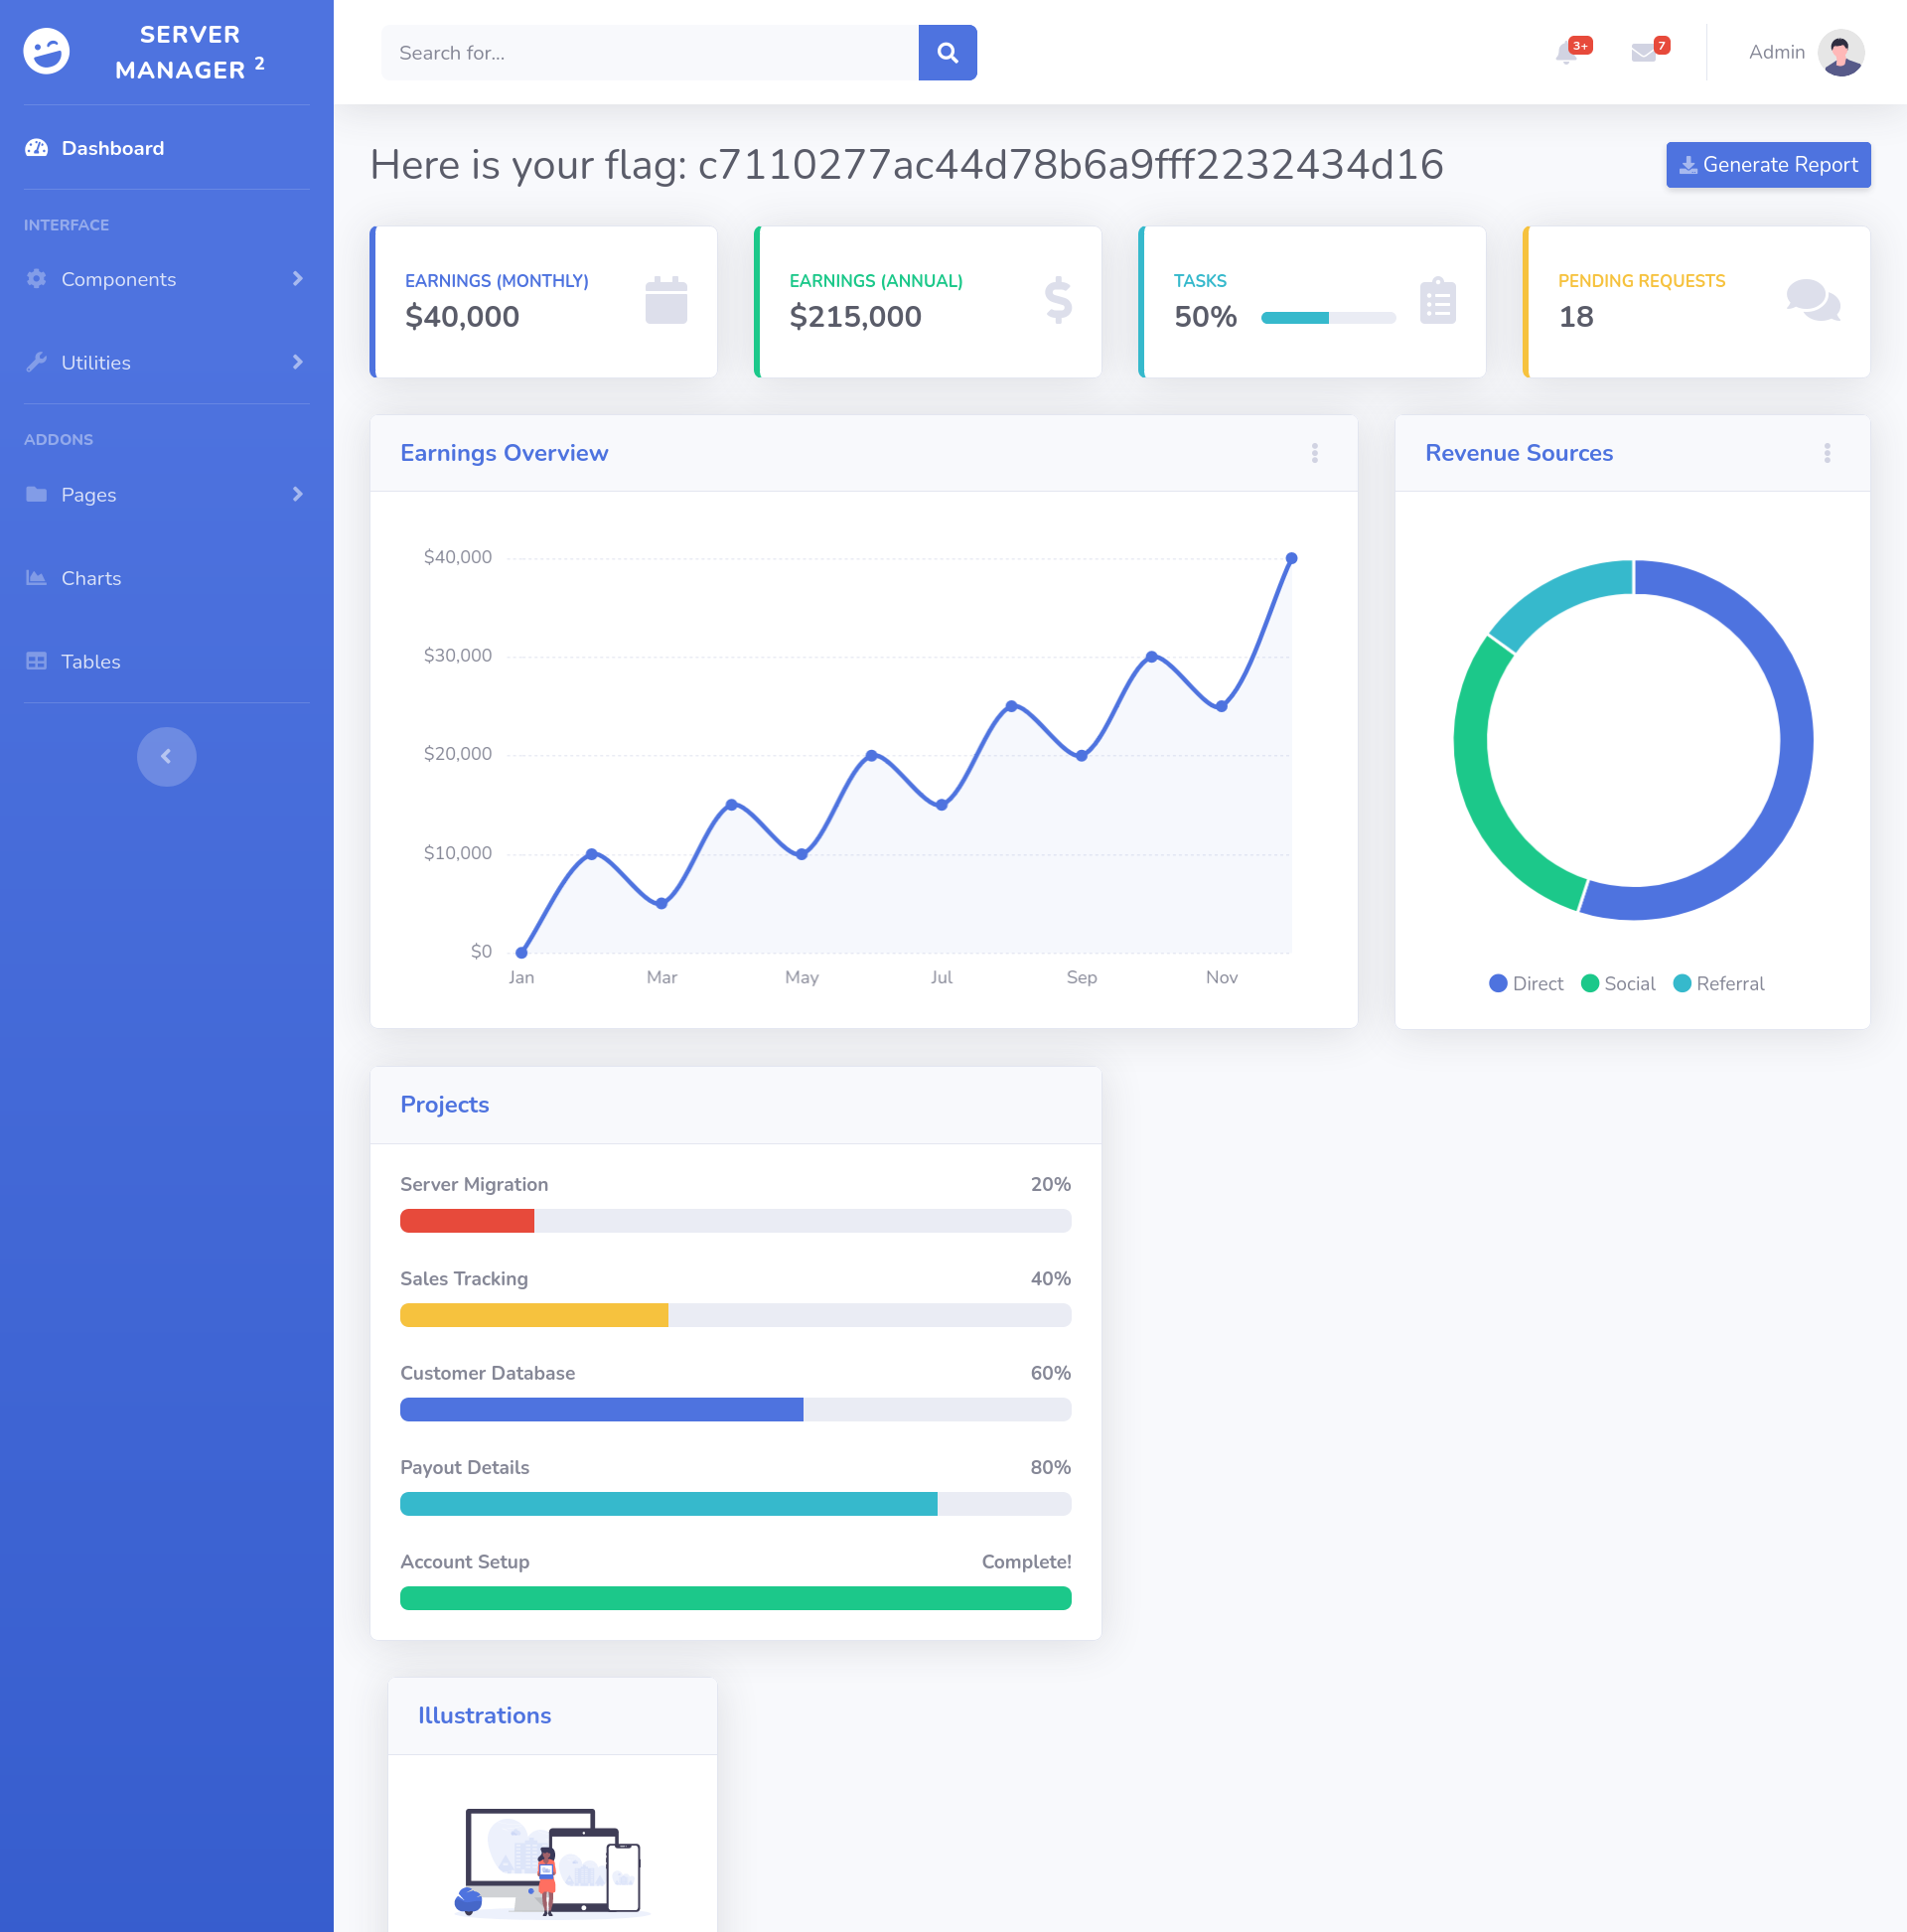
\includegraphics[scale=0.1]{flag.png}
\centering
\end{figure}

We found the flag.


\begin{thebibliography}{00}

\bibitem{gobuster} Oj. “Gobuster: Directory/File, DNS and VHost Busting Tool Written in Go.” GitHub, \url{https://github.com/OJ/gobuster/releases/tag/v3.6.0}.
\bibitem{seclists} Daniel Miessler. “SecLists Is the Security Tester’s Companion. It’s a Collection of Multiple Types of Lists Used during Security Assessments, Collected in One Place. List Types Include Usernames, Passwords, Urls, Sensitive Data Patterns, Fuzzing Payloads, Web Shells, and Many More.” GitHub, \url{https://github.com/danielmiessler/SecLists/releases/tag/2023.2}.

\end{thebibliography}
\vspace{12pt}


\end{document}